% 图 27.2 —— 由 `checks/emit_hand.py` 自动拼出（probe 精测 + prims2 图元分解）
%%
% ⚠ 这是**稿子不是成品**：跑 `checks/checkhand.py 27.2` 看指标 + 看叠合图。
%%
%% ⚠ 待核：
%   · 本图 probe 报出阴影族 1 个 —— **本脚本不生成阴影**（要照原书手写）；prims2 的 strokes 里可能含阴影线，核对时留意别画重
%   · 可疑字形 2 项（空心圈 ⊙ 常被认成字母 o）—— 见文件末
%%
\documentclass[12pt]{standalone}
\usepackage{fontspec}
\setsansfont{Arial}
\newfontfamily\mfallback{DejaVu Sans}
\usepackage{tikz}
\begin{document}
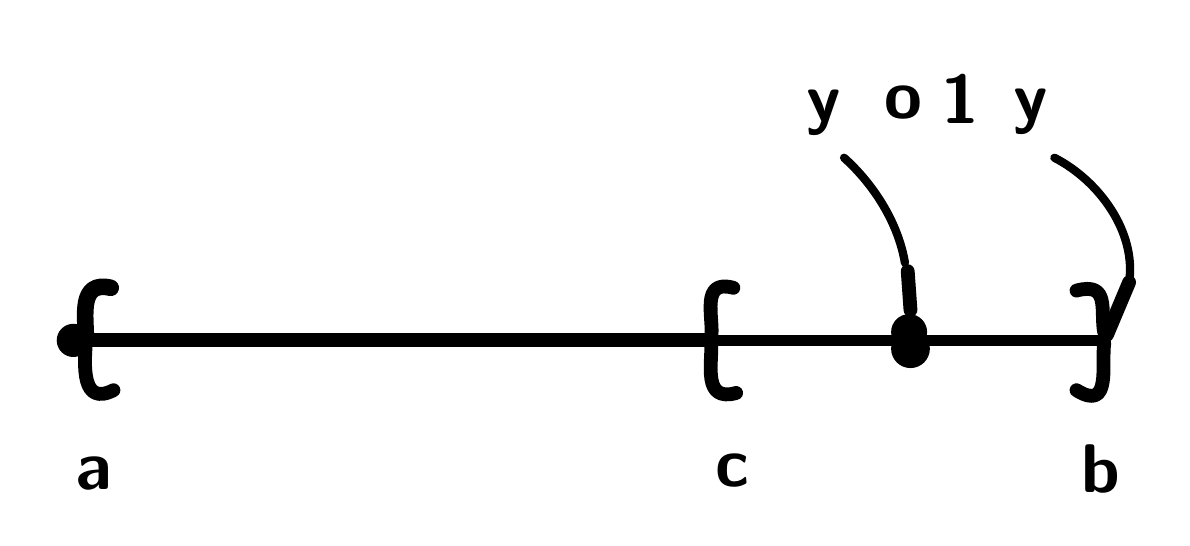
\begin{tikzpicture}[x=1pt, y=-1pt, line width=4.0pt, line cap=round, line join=round]

  %% ════ 填充区（prims2 的 fills）════

  %% ════ 直线段（prims2 的 strokes）════
  \draw[line width=4.0pt] (248.0,113.0) -- (388.0,113.0);
  \draw[line width=5.0pt] (22.0,113.0) -- (246.0,113.0);
  \draw[line width=5.0pt] (390.0,111.0) -- (398.0,92.0);
  \draw[line width=5.0pt] (318.0,88.0) -- (319.0,102.0);

  %% ════ 曲线（prims2 的 curves —— 三段式，坐标同为 (y,x)）════
  \draw[line width=5.0pt] (21.0,114.0) .. controls (20.5,121.6) and (19.3,137.0) .. (31.0,131.0);
  \draw[line width=5.0pt] (389.0,110.0) .. controls (387.5,102.5) and (391.3,91.7) .. (379.0,95.0);
  \draw[line width=3.0pt] (317.0,85.0) .. controls (314.6,70.6) and (305.8,56.7) .. (295.0,47.0);
  \draw[line width=6.0pt] (30.0,94.0) .. controls (18.3,91.2) and (21.1,104.8) .. (21.0,112.0);
  \draw[line width=5.0pt] (389.0,114.0) .. controls (387.9,121.6) and (391.8,139.0) .. (379.0,131.0);
  \draw[line width=5.0pt] (255.0,94.0) .. controls (242.9,90.7) and (248.0,104.9) .. (247.0,112.0);
  \draw[line width=3.0pt] (398.0,92.0) .. controls (400.7,73.9) and (387.2,55.3) .. (371.0,47.0);
  \draw[line width=5.0pt] (247.0,114.0) .. controls (247.4,121.4) and (243.8,135.4) .. (256.0,132.0);

  %% ════ 实心点 ════
  \fill (16.5,113.0) circle (6.0);
  \fill (318.5,110.0) circle (6.5);
  \fill (319.0,116.0) circle (7.0);

  %% ════ 标签（probe 直接给的 \node 行）════
  %% ⚠ 全部补了 fill=white：文字在最上层，否则与曲线交叉干扰
     \node[anchor=center,inner sep=0pt,fill=white,font=\fontsize{31.4}{39.2}\selectfont] at (316.3,27.1) {\textsf{\textbf{\textit{o}}}};   % box(307,17,17,17)
     \node[anchor=center,inner sep=0pt,fill=white,font=\fontsize{27.4}{34.2}\selectfont] at (337.2,26.0) {\textsf{\textbf{1}}};   % box(329,17,10,17)
     \node[anchor=center,inner sep=0pt,fill=white,font=\fontsize{29.8}{37.3}\selectfont] at (362.7,30.2) {\textsf{\textbf{\textit{y}}}};   % box(354,17,17,23)
     \node[anchor=center,inner sep=0pt,fill=white,font=\fontsize{29.2}{36.4}\selectfont] at (287.7,30.7) {\textsf{\textbf{\textit{y}}}};   % box(279,18,17,22)
     \node[anchor=center,inner sep=0pt,fill=white,font=\fontsize{30.0}{37.5}\selectfont] at (387.8,159.2) {\textsf{\textbf{\textit{b}}}};   % box(378,147,17,22)
     \node[anchor=center,inner sep=0pt,fill=white,font=\fontsize{29.4}{36.8}\selectfont] at (254.7,160.0) {\textsf{\textbf{\textit{c}}}};   % box(247,150,14,17)
     \node[anchor=center,inner sep=0pt,fill=white,font=\fontsize{32.0}{40.0}\selectfont] at (24.1,161.1) {\textsf{\textbf{\textit{a}}}};   % box(15,151,16,17)

  % 钉死画布：否则超出的图元/控制点会把页面撑大，1:1 回比就失准
  \pgfresetboundingbox
  \path[use as bounding box] (0,0) rectangle (410,177);
\end{tikzpicture}
\end{document}

% ⚠ 待核清单（probe 拿不准，人眼过一遍）：
%   · 可疑字形：\node[anchor=center,inner sep=0pt,font=\fontsize{31.4}{39.2}\selectfont] at (316.3,27.1) {\textsf{\textbf{\tex
%   · 未识别/跳过：⑤ 跳过/未识别的字形
